\section{Main theorem}

\begin{frame}
The main lemma we need is that the total swirling is 0. We will use four facts:
\begin{itemize}
\item The fibers \( T_i \) are torsors and they are pointed.
\item A sum over faces is a sum over edges, and each edge is appears once in each direction.
\item \( S^1 \) is commutative.
\item Hence there is total cancellation.
\end{itemize}
\end{frame}

\begin{frame}{Vector fields when the tangent bundle is principal}
\begin{columns}
\begin{column}{0.2\textwidth}
\begin{tikzcd}[ampersand replacement=\&, column sep=small]
  \&\& \& {T_1} \\
  \&\&\& {T_{13}T_{32}T_{21}X_1} \\
  \&\& \& {T_{13}T_{32}X_2} \\
  \&  \&  \& {T_{13}X_3} \\
  \&\& \& {X_1}
  \arrow["{\alert{T_{13}T_{32}X_{21}}:}", equals, from=3-4, to=2-4]
  \arrow["{\alert{T_{13}X_{32}}:}", equals, from=4-4, to=3-4]
  \arrow["{\alert{X_{13}}:}", equals, from=5-4, to=4-4]
\end{tikzcd}
\end{column}
\begin{column}{0.8\textwidth}
\begin{itemize}
\item Def: \( \alpha_i\defeq s(-,X_i):T_i\simto S^1 \) (\alert{trivialization on 0-skeleton}).
\item Def: \( \rho_{ji}\defeq \alpha(T_{ji}(X_i)) \) is \alert{the rotation of \( T_{ji} \)}.
\item Lemma: \( \rho_{ij}=\rho_{ji}^{-1} \) because \( \rho_{ij}\cdot\rho_{ji}\cdot X_j=_{T_j}\rho_{ij}\cdot T_{ji}X_i=_{T_j}T_{ji}(\rho_{ij}\cdot X_i)=_{T_j}T_{ji} T_{ij} X_j=_{T_j}X_j \).
\item Now to paths:
\item Define \( \sigma_{ji}\defeq s(X_{ji}, X_j):\rho_{ji}=_{S^1}\base, \) a path from a rotation to the identity.
\item Paths of the form \( a=_{S^1}\base \) can be multiplied: \( \mu:(a=\base)\times (b=base)\to \mu(a, b)=base \), \( \mu(p, q)=\mu(p, b)\cdot q. \)
\item So if \( X_\tot = X_{21}\cdot X_{32}\cdot\cdots \) then \( \alpha(X_\tot)=\sigma_{21}\cdot\sigma_{32}\cdot\cdots \).
\item Lemma: \( \apd(\refl)=\refl\implies X_{ij}\cdot T_{ij}X_{ji}=\refl_{X_i}\implies\sigma_{ij}\cdot\sigma_{ji}=\refl_{\base} \).
\item We assume that summing over faces visits every edge once in each direction.
\item \( S^1 \) is commutative, hence complete cancellation.
\end{itemize}
\end{column}
\end{columns}
\end{frame}


\begin{frame}{Consequence}
Yeah.
\end{frame}

\begin{frame}{Classical proof}
\begin{columns}
\column{0.5\textwidth}
\vspace{12pt}
\begin{figure}
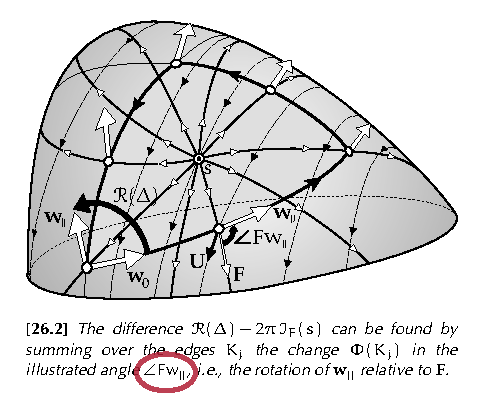
\includegraphics[width=0.9\textwidth]{figs/needham_triangle_circ.pdf}
\caption{{Needham,~T. (2021) Visual Differential Geometry and Forms.}}
\end{figure}
\column{0.5\textwidth}
\vspace{-12pt}
\begin{itemize}
\item The classical proof is discrete-flavored.
\item ``\( \angle Fw_{||} \)'' looked a lot like a pathover.
\item Hopf's \( \Phi \) is defined on edges, not loops. We imitated that too.
\end{itemize}
\end{columns}
\end{frame}
